\section{DICOM en pratique}

\frame
{
	\frametitle{Anonymisation}
	\begin{itemize}
		\item Utilisation d'images cliniques pour la recherche ou l'enseignement.
		\item Fichiers mis \`a disposition du public.
		\item N\'ecessit\'e d'anonymat : suppression des informations personnelles permettant d'identifier le patient.
		\begin{itemize}
			\item PatientsName (0010,0010)
			\item PatientID (0010,0020)
			\item PatientBirthDate (0010,0030)
			
			$\rightarrow$ de type 1 : \`a remplacer, pas supprimer !
			\item ReferringPhysicianName (0008,0090)
			\item etc.
			\item Potentiellement plus de 250 champs \`a supprimer ou \`a vider !
		\end{itemize}
	\end{itemize}
}

\frame
{
	\frametitle{Achat d'un \'equipement}
	\begin{enumerate}
		\item Avant l'achat, soumission de l'appel d'offre :
		\begin{itemize}
			\item D\'efinition du sc\'enario de travail souhait\'e.

                Exemple : les images brutes export\'ees pourront \^etre r\'eutilis\'ees \emph{a posteriori}.
			\item R\'edaction du cahier des charges DICOM.
			\begin{itemize}
				\item Pr\'eciser le niveau d'exigence de DICOM.
				
				$\rightarrow$ faire appel \`a un consultant ou \`a des coll\`egues,
				
				$\rightarrow$ ou acqu\'erir le savoir-faire en interne.
				\item Demander le Document de Conformit\'e DICOM (DICOM Conformance Statement).
			\end{itemize}
		\end{itemize}
		\item Acceptation protocol\'ee.
		\begin{itemize}
			\item V\'erification de DICOM.
			\item V\'erification du/des sc\'enario/ii requis.
			\item Tests.
		\end{itemize}
	\end{enumerate}
}

\frame
{
	\frametitle{DICOM Conformance}
	\begin{itemize}
		\item Le standard pr\'evoit un document "DICOM Conformance Statement" dont le plan et la structure sont pr\'ed\'efinis.
		\item Par ce document, le fournisseur pr\'ecise le niveau de conformit\'e de son \'equipement au standard DICOM.
		\begin{itemize}
			\item Applicable sur chaque mod\`ele, chaque version.
			\item Le document suit un plan pr\'evu dans le standard.
			\item Liste des SOP Class support\'ees et des r\^oles assur\'es (SCU, SCP).
		\end{itemize}
	\end{itemize}
}

\frame
{
	\frametitle{Exemple de DICOM Conformance Statement}
}

\frame
{
	\frametitle{Services \`a demander}
	Exemples typiques de services DICOM \`a exiger pour un scanner :
	\begin{itemize}
		\item Worklist (SCU) : Import de la liste de patients.
		\item Store : envoi des images par r\'eseau
		\begin{itemize}
			\item Envoi : modalit\'es (SCU) : \textbf{CT}.
			\item R\'eception (SCP) : \textbf{CT}, \textbf{IRM}.
		\end{itemize}
		\item Print (SCU) : envoi des images pour impression
	\end{itemize}
	
	\begin{center}
		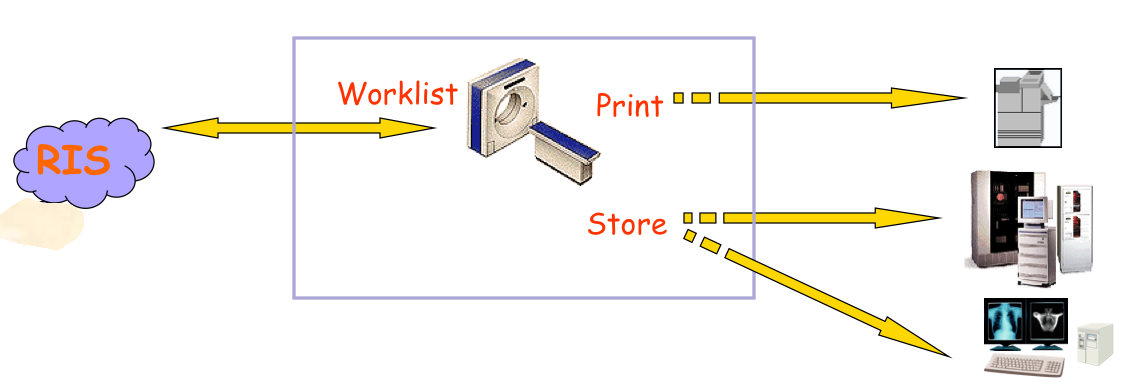
\includegraphics[width=\linewidth]{./figures/services-ct.png}
	\end{center}

}

\frame
{
	\frametitle{\'Equipements non standards}
	
	\begin{itemize}
		\item Int\'egrer dans un workflow DICOM : installer une passerelles de conversion.
		
		\begin{center}
			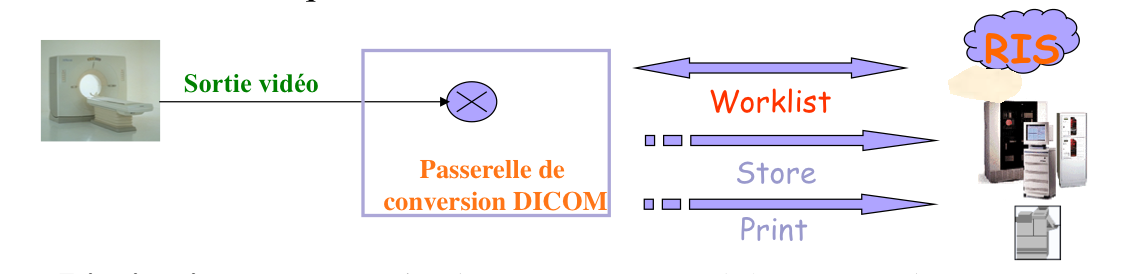
\includegraphics[width=\linewidth]{./figures/passerelle.png}
		\end{center}
		\item Limitation : images stock\'ees en mode Secondary Capture (IOD le plus simple de DICOM), les donn\'ees d'acquisition des images sont perdues.
	\end{itemize}
}

